% Acknowledgments must be written in complete sentences. Do not use direct address. For example, instead of "Thanks, Mom and Dad!", you should say "I thank my parents".

Making it to this point in my academic career was only possible because of the many two- and four-legged blessings in my life.
I therefore give my endless gratitude\ldots

To my high-energy physics mentors, Professors Andrey Korytov and Guenakh Mitselmakher, for granting me this one-of-a-kind opportunity to do \emph{real particle physics} at CERN as part of the CMS collaboration.
To Prof. Darin Acosta for spending countless patient hours of physics discussion with me and the other students during our ``CMS Office Hours'' and for being a committee member.
To Prof. Konstantin Matchev for keeping a relaxed and encouraging eye on me since the very beginning of this journey and also for serving on my committee.
To Professors Alina Zare and John Yelton for serving as crucial members on my committee.

To Dr. Filippo Errico for his focus, selflessness, and patience in leading the Higgs boson mass measurement and for doing much of the heavy lifting.
If not for Filippo, no doubt this analysis would never see its end.
To Dr. Lucien Lo for leading the dilepton mass resonance analysis and for showing me the beauty of Python in his laid-back way.
To Brendan Regnery and Dr. Bhargav Joshi, the gentlemen who paved my way into and through the world of CMS with their kindness and optimism.
To Dr. Hualin Mei for laying the initial framework for the 2016 Higgs boson mass measurement.
To Dr. Xunwu Zuo for his willingness to share his CMS knowledge with me.
To the CMS researchers who took me under their wing while at CERN: Dr. Christian Schnaible, Dr. Katerina Kuznetsova, Nick Manganelli, Dr. Riju Dasgupta, and Sasha Golunov.

To my comrades for showing me what it takes to survive the core courses: Dr. Atul Divakarla (Atool), Dr. Brendan O'Brien (Robo-son), Dr. Daniel Guerrero (donYELL), Haechan Park, \textgreek{Ιωάννης Μιχαλολιάκος}, Dr. Soham Kulkarni, and Dr. Vladimir Martinez (Vladimort), \ie the \emph{Slim Gyms}. Stay strong, boys.
To Dr. Alex Schachtner for being the example I strive to be.
To Hoda Akl for her perfectly pertinent gifts, most notable of which is still the practice of Essentialism.
To Mayar Shahin for gracefully co-directing the Physics Graduate Community at the drop of a hat.
To Chuck Parks (the Meter Stick Marauder) for the unwavering help he selflessly gives to any student in need, especially when the right tool is a good ol' trigonometric substitution.
To Rebika Makaju for her personality, which is just as nourishing as her food.
To Ammar Jahin for his dependably lighthearted support.
To Shubha Bhaumik for being honest and open with me about the importance of maintaining mental and physical health.
To Dr. Prasanth Shyamsundar for his contagious enthusiasm concerning anything physics.
To Dr. Adamya Goyal for his many lessons on physics and friendship.

To the folks who not only made terrific contributions to our 2019--2021 CMS Office Hours but who also patiently listened to me stumble over myself for hours as I tried to explain particle physics:
Ari Gonzalez, Arun Madhu, Cris Caballeros, Evan Koenig, Jeremiah Anglin, John Rötter, Neha Rawal, Nik Menendez, and Sean Kent.
To my mentee, Matthew Dittrich, for his many conversations which rekindled my love for particle physics and for heeding my advice.

To the ultra-efficient Pam Marlin, who is the lifeblood of the physics department.
To Connie (Nana), Madel, and Jessica, for stocking us up on supplies at a moment's notice and for handling those piles of receipts.
To the computer staff, David Hansen and Clint Collins, who manage to keep their cool amidst never-ending tech crises.
To the indefatigable Anna Pardo and Stacy Wallace for help with the editorial and submission processes, along with their motivational support.
To Frank from the custodial staff, whose smile can cheer up the most morose of men.

To my physics pham, who remind me just how fun the subject can be:
Cameo Lance, who lives fully and fearlessly;
Gabe Fuentes (Gabey Babey), who laughs anything off;
Morgan Walker (``OK, Morgan''), who makes sense of it all;
Dr. Noah Steinberg, who speaks physics directly into your brain;
Derek Woods, who anthropomorphizes the adage ``work smarter---not harder'';
and April Woods, who dabbles in everything and does it well.

To my mentor, Sheldon Friedman, and his wife, Rita Friedman (Rosenzweig), who invested their encouragement, love, and optimism in me at a very young and impressionable age.
Their return on that investment has manifested in the very form of success which Sheldoni always promised: \emph{the realization of a worthwhile, predetermined goal}\ldots a Ph.D. in particle physics!
%  through their chose to invest in my success at a very young age.  % TODO %---\emph{the realization of a worthwhile, predetermined goal of earning a Ph.D.}---at a very young age.
% That success has manifested itself in exactly the form Sheldoni always said it would: \emph{the realization of a worthwhile, predetermined goal}\ldots a Ph.D. in particle physics!
% With their continued , I realized this worthwhile, predetermined goal of earning a Ph.D. in particle physics.
%  have obtainedearned 
% Fast forward 20 years and I've now earned this Ph.D. degree is yet another form of success which Sheldon defines as: .
To Sheldon's best friend, Dr. Bernard Khoury, whose reputation and prose set me on this journey in the first place and in whose footsteps I follow.
To the high school teachers who laid the foundation of my higher education and encouraged me to go all the way: Mrs. Beth Sweet, Mrs. Marie Girardeau (\emph{requiescas in pace, Magistra}),  Mr. Tim Allen, and Mr. Tom LaPointe.

To my quantum fluctuation, my wife Suzanne Rosenzweig, for showing me that dreams do come true and that the only thing constant in life is change.
To my mother and father, Vicki and John, who always reassured me that I could achieve anything I put my mind to. Sleep peacefully, Mom.
To my Auntie Rachel and Uncle Yuri---my biggest cheerleaders---with whom together we think \emph{kvell}.
To my siblings, Alex, Ryan, Devin, Jace, and Claudia, who regularly reminded me that life existed outside of grad school.
To Grandmommy and Granddaddy for demonstrating what unconditional love looks like.
To Jennifer Wyckoff for teaching me long division; little did she know that she planted the math seed all those years ago!
To Mark Wyckoff for showing me that life is meant to be lived in whatever way you choose.
To Rob and Amy Buckley for taking every chance they get to remind me how much pride they have for me.
To Jen and Sarah Buckley for sharing their sanctuaries with me in which we held transformative conversations during the final days of this dissertation writing.
To Jayson Margush, who 3D-printed an incredibly impressive, pull-apart model of CMS! My committee was \emph{quite} excited to play with it.
To Mr. Tankaboy: DO you\ldots \emph{want some food?}

To the boys who have been there since the beginning: Jish, Willis, The Witch Dr. Shane Reilly-Rogers, Zacman, Duck, and Marcus Jackson for their clever competition and continual camaraderie which has pushed me to earn this degree.
To the many moms who generously gave relentless support during the darkest times and unequivocal love during the brightest times:
Cyndi Reilly-Rogers, Dawn Hood, Kayla Rynor, Margaret Sherrill, Silet Wiley.
To my Polish roommates in Saint-Genis-Pouilly for showing me what home away from home feels like: Bartoszek, Dziadziuś, Karolina, and Sandruśa.
To Adina Hoffman---the first to graduate from the ``Dissertation Station''---for sharing her Gaggia Brera and her Alain Brera with me.
To Carina Dorothy Krehl for showing me the beauty of sobriety and of self.
To Wim Hof for teaching me what power and life exists in our very breath.
To my generous and supportive neighbors who fed me food when physics just wasn't sufficiently nutritious: Elizabeth Buckhalter, Hugh Pritchett, Joe Klubertanz, Little Linton, and Robert Jenkins.

To the Physics Tree which stood in the north lawn of NPB (Fig.~\ref{fig:phys_tree}) as a symbol of strength, beauty, and life for several centuries before anyone reading this paper was even born.
September 11, 2017 was a portentous day as Hurrican Irma trembled the entirety of the New Physics Building (NPB).
In the middle of the night, around 02:15, the northern forked trunk of the Physics Tree had fallen towards the northwest, leaving its southern half to stand and bear the tempest alone.
By 04:30, Irma's wild whirring winds worsened and the racket of ripping roots resounded throughout the western corridor of NPB.
There I stood in that frozen moment---awestruck, speechless, and alone---watching the magnificent remnant trunk \emph{fall}\ldots helplessly\ldots directly southward towards NPB.
What could have been the destruction of our sanctuary was instead a gentle grazing against its northern windows, without a single window shattered, where, there, the Physics Tree gracefully laid itself to rest once and for all.

Finally, to Existence itself, for this unpredictable, lovely blip of an experience we call Life.
%%%%%%%%%%%%%%%%%%%%
\begin{multiFigure}
    \centering
    \addFigure{0.53}{figures/bigtree_pam.jpeg}
    \addFigure{0.43}{figures/bigtree_down.JPG}
    % 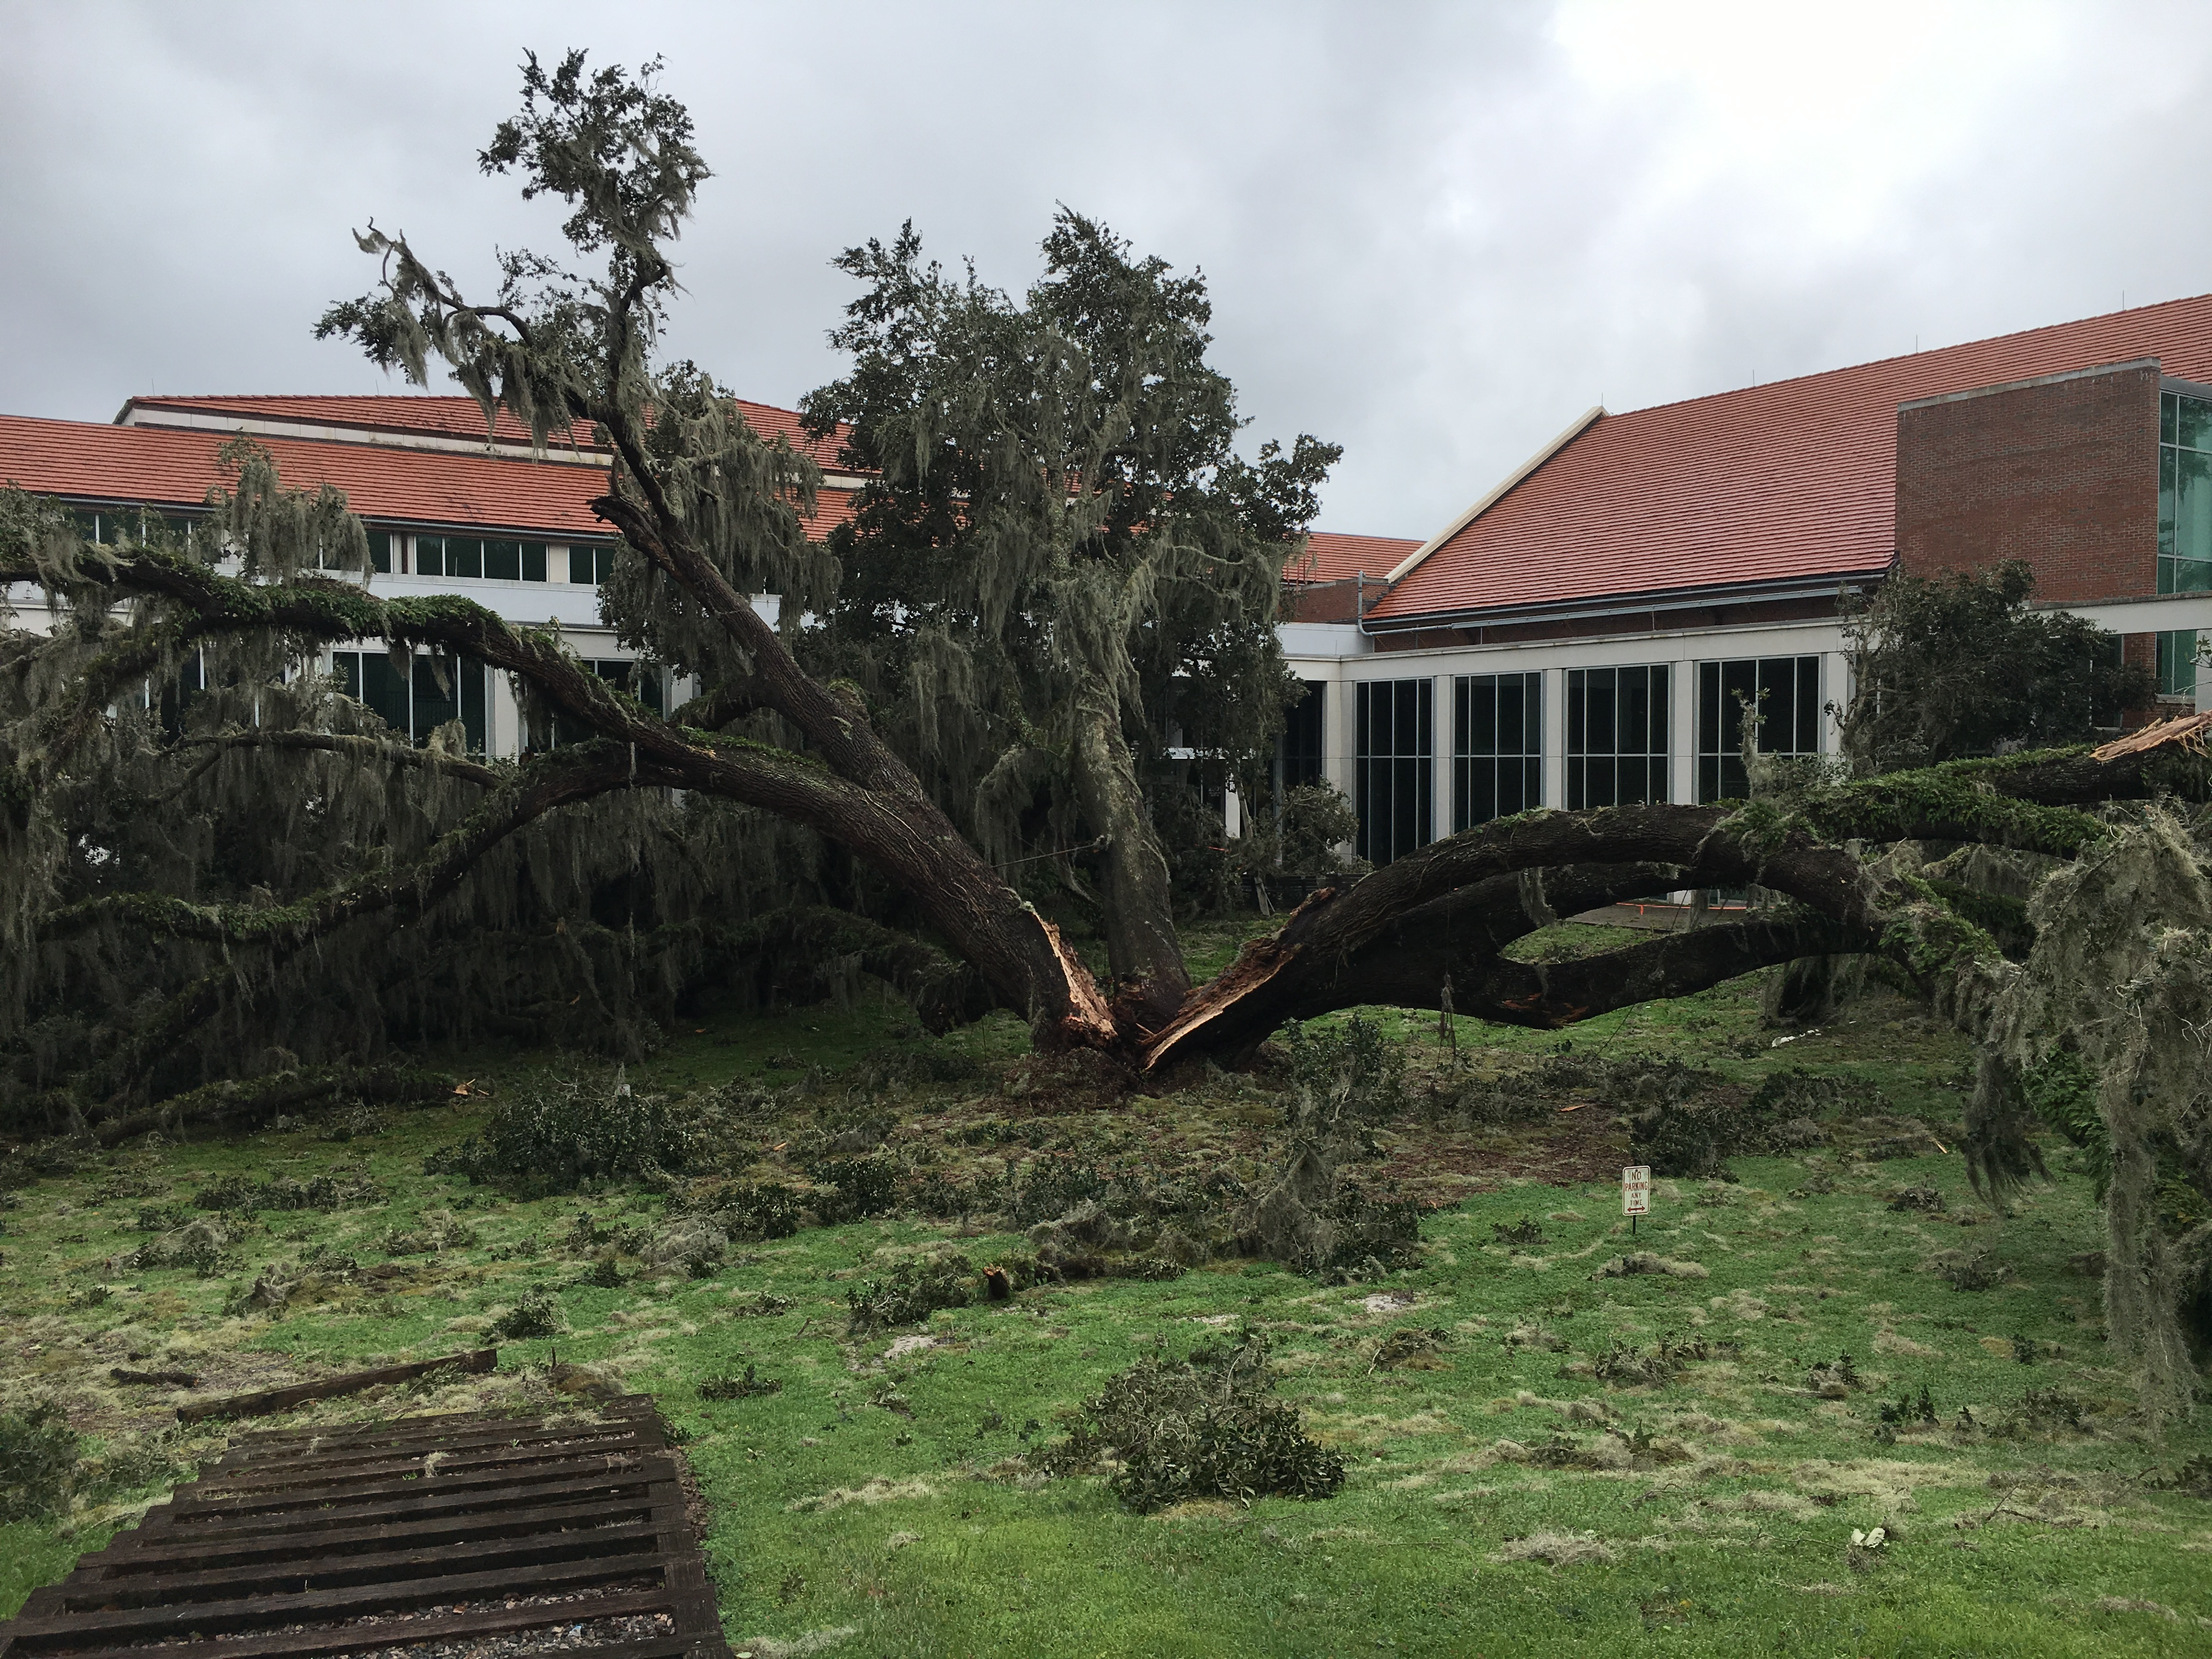
\includegraphics[height=5cm]{bigtree_down.JPG}
    \captionof{figure}
        [The Physics Tree before and after Hurricane Irma]
        {The Physics Tree in front of NPB, as viewed from Museum Road looking south.
        \;A) Before Hurricane Irma. Photo courtesy of Pam Marlin.
        \;B) After Hurricane Irma (September 11, 2017). Photo courtesy of the author.
        }
    \label{fig:phys_tree}
\end{multiFigure}
%%%%%%%%%%%%%%%%%%%%